\documentclass[12pt, a4paper]{article}

\usepackage{fullpage}
\usepackage{latexsym}
\usepackage{amsfonts}
\usepackage{amssymb}
\usepackage{graphicx}
\usepackage{amsmath}
\usepackage{float}
\usepackage{subcaption}

\pagestyle{empty}

\begin{document}

\title{{AMATH 568\\
Advanced Differential Equations}\\
{\bf \Huge Homework 4}}

\author{Lucas Cassin Cruz Burke}

\date{Due: February 3, 2023}

\maketitle

\begin{enumerate}

\item Consider the weakly nonlinear oscillator: 

$$\frac{d^2 y}{dt^2} + y + \epsilon y^5 = 0$$

with $y(0)=0$ and $y'(0)=A>0$ and with $0 < \epsilon \ll 1$.

\begin{enumerate}
    \item Use a regular perturbation expansion and calculate the first two terms.

    \textbf{Solution:} Let $y=y_0 + \epsilon y_1 + \dots$. Then our ODE becomes

    \begin{align*}
        y_0'' + \epsilon y_1'' + y_0 + \epsilon y_1 + \epsilon y_0^5 + \mathcal{O}(\epsilon^2) = 0
    \end{align*}

    Looking at the $\mathcal{O}(1)$ terms, we have

    $$y_0''+y_0=0 \Rightarrow y_0=A\sin t+B\cos t$$

    Applying the boundary condition $y_0(0)=0$ and $y_0'(0)=A$ we find our first order solution to be

    $$y_0(t) = A \sin t$$

    Next, we look at the $\mathcal{O}(\epsilon)$ terms. Plugging in our solution for $y_0$, we have

    \begin{align*}
        y_1'' + y_1 +A^5 \sin^5 t = 0 \Rightarrow y_1'' + y_1 = -A^5 \sin^5 t
    \end{align*}

    For the homogeneous problem, we have the general solution $y = c_1\sin(t) + c_2\cos(t)$. For the particular solution we use Mathematica and find

    $$y_1(t) = \frac{-5}{128} A^5 \sin(3t) + \frac{1}{384} A^5 \sin(5t) + \frac{5}{16} A^5 t\cos(t) + c_1 \sin(t) + c_2 \cos(t)$$

    From the boundary condition $y_1(0)=0$ we see that $c_2=0$, and from the boundary condition $y_1'(0)=0$ we have 

    $$y_1'(0) = \frac{-15}{128} A^5 + \frac{5}{384} A^5 + \frac{5}{16}A^5 + c_1 = 0 \Rightarrow c_1 = \frac{-5}{24}A^5$$

    Hence, we may write our second order correction term as 

    $$y_1(t) = \frac{-5}{128} A^5 \sin(3t)+\frac{1}{384}A^5 \sin(5t) + \frac{5}{16} A^5 t\cos(t) - \frac{5}{24}A^5 \sin(t)$$

    Note that, since $\sin^5 t$ is not orthogonal to the null-space, we have secular growth terms $\sim t \cos(t)$. 

    Combining our $y_0$ and $y_1$, we find the following approximate solution from the regular expansion method:

    $$y(t) = A \sin t + \epsilon \left[ \frac{-5}{128} A^5 \sin(3t)+\frac{1}{384}A^5 \sin(5t) + \frac{5}{16} A^5 t\cos(t) - \frac{5}{24}A^5 \sin(t) \right] + \mathcal{O}(\epsilon^2)$$

    \item Determine at what time the approximation of part (a) fails to hold.

    \textbf{Solution:} We note that there is a secular growth term in $y_1(t)$ given by

    $$\frac{5}{16} A^5 t\cos(t)$$

    This term will grow linearly with time, and so for large time-scales our assumption that $\epsilon y_1(t)$ is a small correction begins to break down. In particular, we see that our approximation fails when 

    $$t \sim \frac{1}{A^5} \frac{1}{\epsilon}$$

    \item Use a Poincare-Lindstedt expansion and determine the first two terms and frequency corrections.

    \textbf{Solution:} We now expand $y(t)$ in terms of slow time $\tau$.

    \begin{align*}
        y(t) = y_0(\tau) + \epsilon y_1(\tau) + \mathcal{O}(\epsilon^2) && \tau = \omega t = (\omega_0 + \epsilon \omega_1 + \dots) t
    \end{align*}

    Making the change of variables from $t \rightarrow \tau$ results in

    \begin{align*}
        y_{tt} + y + \epsilon y^5 = 0 && \Rightarrow && \omega^2 y_{\tau \tau} + y + \epsilon y^5 = 0
    \end{align*}

    Plugging in our power series expansions for $y$ and $\omega$ gives us, to $\mathcal{O}(\epsilon)$, 

    \begin{align*}
        (\omega_0^2 + 2 \epsilon \omega_0 \omega_1)(y_{0\tau\tau} + \epsilon y_{1\tau\tau}) + y_0 + \epsilon y_1 + \epsilon y_0^5 = 0
    \end{align*}

    To $\mathcal{O}(1)$ we have

    \begin{align*}
        \omega_0^2 y_{0\tau\tau} + y_0 = 0 && \Rightarrow && y_0(\tau) = c_1 \sin(\tau/\omega_0) + c_2 \cos(\tau/\omega_0)
    \end{align*}

    The Dirichlet boundary condition at $t=0$ means that $c_2=0$, while the Neumann boundary condition means that

    \begin{align*}
        \frac{c_1}{\omega_0} = A && \Rightarrow && c_1 = A \omega_0
    \end{align*}

    Hence our first order solution comes out to

    $$y_0(\tau) = A\omega_0 \sin(\tau/\omega_0)$$

    We now continue to $\mathcal{O}(\epsilon)$. Here we have

    $$\omega_0^2 y_{1\tau\tau} + y_1 = -2\omega_0\omega_1 y_{0\tau\tau} - y_0^5 = 2A\omega_1\sin(\tau/\omega_0) - A^5 \omega_0^5 \sin^5(\tau/\omega_0)$$

    For the homogeneous problem we have the solution $y = c_1 \sin(\tau/\omega_0) + c_2 \cos(\tau/\omega_0)$

    and for the particular solution, we turn to Mathematica.

    \begin{align*}
        y_1(\tau) &= -\frac{7}{96}A^5\omega_0^5\sin(\tau/\omega_0)\cos(2\tau/\omega_0) + \frac{1}{192}A^5\omega_0^5\sin(\tau/\omega_0)\cos(4\tau/\omega_0) \\&+ \frac{5}{16}A^5\omega_0^4\tau\cos(\tau/\omega_0) - A\omega_1\tau\cos(\tau/\omega_0)/\omega_0 + c_1\sin(\tau/\omega_0) + c_2\cos(\tau/\omega_0)
    \end{align*}

    In order to avoid secular growth terms, we see that the frequency correction $\omega_1$ must satisfy

    \begin{align*}
        \frac{5}{16} A^5 \omega_0^4 - A\omega_1 = 0 && \Rightarrow && \omega_1 = \frac{5}{16} A^4 \omega_0^4
    \end{align*}

    Lastly, the boundary conditions require that $c_2=0$, and that 

    \begin{align*}
        y_1'(0) = - \frac{7}{96} A^5 \omega_0^4 + \frac{1}{192} A^5 \omega_0^4 + c_1/\omega_0 = 0 &&
        \Rightarrow && c_1 = \frac{13}{192} A^5 \omega_0^5
    \end{align*}

    And so the complete $\mathcal{O}(\epsilon)$ correction can be written down as 

    $$y_1(\tau) = \frac{A^5 \omega_0^5}{192} \sin(\tau/\omega_0) \left( -14 \cos(2\tau/\omega_0) + \cos(4\tau/\omega_0) + 13 \right)$$

    We can now put together our full approximate accurate solution. We will let $\omega_0=1$ to look for $2\pi$-periodic solutions. Then $\tau = (1 + 5\epsilon A^4/16)t$. We then have

    \begin{align*}
        y(t; \epsilon) &= A \sin[(1 + 5\epsilon A^4/16)t] \\&+ \epsilon \frac{A^5}{192} \sin[(1 + 5\epsilon A^4/16)t]\left( -14 \cos[2(1 + 5\epsilon A^4/16)t] + \cos[4(1 + 5\epsilon A^4/16)t] + 13 \right) \\
        &= A \sin[(1+ 5\epsilon A^4/16)t]\left( 1 - \epsilon \frac{A^4}{48} \sin[(1+5\epsilon A^4/16)t] \left( \cos[2(1+5\epsilon A^4/16)t]-6\right)\right)
    \end{align*}

    
    $$\Rightarrow y(t;\epsilon) = A \sin[(1 + 5\epsilon A^4/16)t)] + \epsilon \frac{A^5}{48} \sin^3(t)(6- \cos(2t))+ \mathcal{O}(\epsilon^2)$$

    \item For $\epsilon = 0.1$, plot the numerical solution (from MATLAB), the regular expansion solution, and the Poincare-Lindstedt solution for $0 \le t \le 20$.

    \textbf{Solution:}

    \begin{figure}[H]
    \centering
    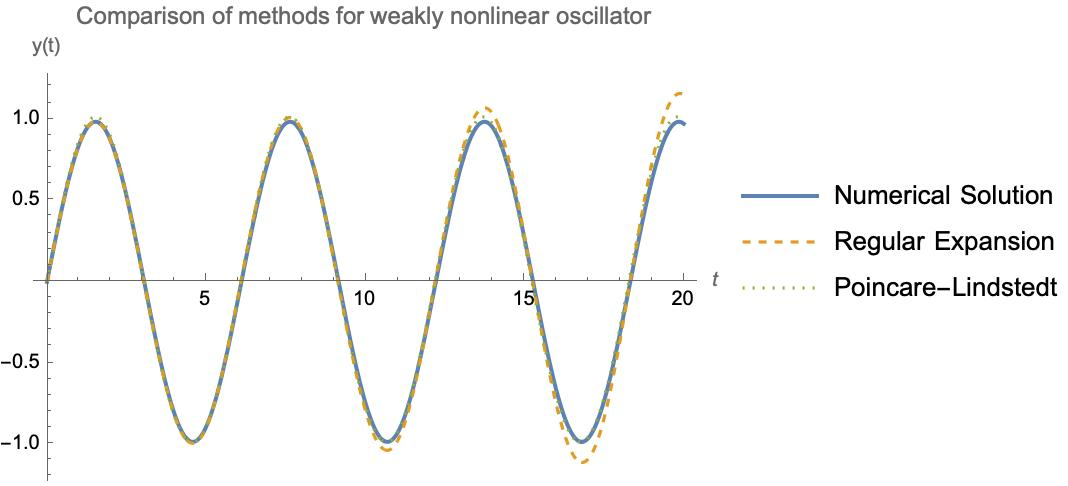
\includegraphics[width=14cm]{Fig1.jpg}
    \caption{Solution comparison for different methods, with $\epsilon=0.1$.}
\end{figure}

\end{enumerate}

\item Consider Rayleigh's equation:

$$\frac{d^2 y}{dt^2} + y + \epsilon \left[ - \frac{dy}{dt}+\frac{1}{3} \left( \frac{dy}{dt}\right)^3 \right] = 0$$

which has only one periodic solution called a "limit cycle" ($0 < \epsilon \ll 1$). Given

$$y(0)=0$$

and 

$$\frac{dy(0)}{dt}=A.$$

\begin{enumerate}
    \item Use a multiple scale expansion to calculate the leading order behavior.

    \textbf{Solution:} Let $y = y_0(t, \tau) + \epsilon y_1(t,\tau) + \mathcal{O}(\epsilon^2)$, where $\tau = \epsilon t$. Then our ODE becomes

    $$y_{0tt} + 2 \epsilon y_{0t\tau} + \epsilon y_{1tt} + y_0 + \epsilon y_1 + \epsilon[-y_{0t} + \frac{1}{3} y_{0t}^3]=0$$

    To $\mathcal{O}(1)$ we have

    \begin{align*}
        y_{0tt}+y_0=0 && \Rightarrow && y_0 = A_0(\tau) \sin t + B_0(\tau) \cos t
    \end{align*}

    By our Dirichlet boundary conditions, we have

    $$y_0(0) = B_0(0) = 0$$
    
    while from our Neumann boundary conditions we have

    \begin{align*}
        y_0'(0) = y_{0t}(0) + \epsilon y_{0\tau}(0) =  A_0(0) + \epsilon B_0'(0)  = A && \Rightarrow && \left\{ \begin{array}{cc}
           A_0(0) = A \\\\
           B_0'(0) = 0
        \end{array}\right.
    \end{align*}
    
    To $\mathcal{O}(\epsilon)$ we have

    \begin{align*}
        y_{1tt} + y_1 &= y_{0t} - 2y_{0t\tau} - \frac{1}{3} y_{0t}^3\\
        &= (A_0 -2A_{0}') \cos t - (B_0-2B_{0}') \sin t - \frac{1}{3}(A_0 \cos t - B_0 \sin t)^3
    \end{align*}

    From Mathematica, we find the solution to this ODE to be

    \begin{align*}
        y_1(t,\tau) = \frac{1}{96} &[-2 \cos (t) \left(48 A_0'+6 B_0 t \left(A_0^2+B_0^2-4\right)+A_0 \left(5 A_0^2+9 B_0^2-24\right)+48 (B_0' t-B_1)\right) \\ &+2 \sin (t) \left(-48 A_0' t-6 A_0^3 t-3 A_0^2 B_0-6 A_0 \left(B_0^2-4\right) t+B_0^3+48 B_1\right) \\ &+B_0 \left(B_0^2-3 A_0^2\right) \sin (3 t) +A_0 \left(A_0^2-3 B_0^2\right) \cos (3 t)]
    \end{align*}

    where $A_1 = A_1(\tau)$ and $B_2 =B_1(\tau)$. To ensure that there are no secular growth terms, we require that $A_0$ and $B_0$ satisfy

    \begin{align*}
        A_0' = \frac{1}{8} A_0(4- A_0^2 - B_0^2) && B_0' = \frac{1}{8}B_0(4- A_0^2 - B_0^2)
    \end{align*}

    Let $G(\tau) = \frac{1}{8} (4-A_0^2 -B_0^2)$. Then $A_0' = A_0 G$ and $B_0' = B_0 G$, and 

    \begin{align*}
        G' &= -\frac{1}{4}(A_0A_0' + B_0B_0') = -\frac{1}{4}(A_0^2 + B_0^2)G \\&= 2G^2 - G
    \end{align*}

    This is a separable equation. Dividing both sides by $2G^2-G$, integrating, and rearranging yields the solution

    $$G(\tau) = \frac{1}{C e^\tau + 2}$$

    where $C>0$ is an integration constant. We can now use this expression to solve for $A_0(\tau)$ and $B_0(\tau)$. We have

    \begin{align*}
        \frac{dA_0}{d\tau} = A_0 G = \frac{A_0}{C e^\tau + 2} \\
        \Rightarrow \int_A^{A_0} \frac{dA_0}{A_0} = \int_0^\tau \frac{d\tau}{Ce^\tau +2}\\
        \Rightarrow \log\left(\frac{A_0}{A}\right) = \frac{\tau}{2} - \frac{1}{2}\log\left(\frac{Ce^\tau +2}{C+2}\right)\\
        \Rightarrow A_0(\tau) = A e^{\tau/2} \sqrt{\frac{C +2}{Ce^{\tau}+2}}    
    \end{align*}

    where we have used $A_0(0)=A$ from our boundary condition. Similarly, we find

    $$B_0(\tau) = B(0) e^{\tau/2} \sqrt{\frac{C +2}{Ce^{\tau}+2}} = 0$$

    since $B_0(0)=0$ from our boundary conditions.

    Having solved for $A_0(\tau)$ and $B_0(\tau)$, we may write down our first order approximate solution as 

    $$y_0(t,\tau) = A\sin (t) e^{\tau/2} \sqrt{\frac{C +2}{Ce^{\tau}+2}}$$\\
    $$\Rightarrow y_0(t) = A\sin (t) e^{\epsilon t/2} \sqrt{\frac{C +2}{Ce^{\epsilon t}+2}}$$

    We note that in the limit $t\rightarrow \infty$ the right-hand side approaches $A \sin(t)$.\\

    \item Use a Poincare-Lindsted expansion and an expansion of $A=A_0 + \epsilon A_1 + \dots$ to calculate the leading-order solution and the first non-trivial frequency shift for the limit cycle.

    \textbf{Solution:} Let 

    \begin{align*}
        y&=y_0(\tau) + \epsilon y_1(\tau) + \dots \\ \tau &= \omega t = (\omega_0 + \epsilon \omega_1 + \dots) t \\ A &= A_0 + \epsilon A_1 + \dots
    \end{align*}

    Then our ODE becomes

    \begin{align*}
        \omega^2 y_{\tau\tau} + y + \epsilon \left[-\omega y_\tau + \frac{1}{3} \omega^3 y_\tau^3 \right] &= 0 \\
        (\omega_0^2 + 2 \epsilon \omega_0 \omega_1)(y_{0}'' + \epsilon y_{1}'') + y_0 + \epsilon y_1 + \epsilon \left[ -\omega_0 y_0' + \frac{1}{3} \omega_0^3 {y_0'}^3\right]  &= \mathcal{O}(\epsilon^2)
    \end{align*}

    Then to $\mathcal{O}(1)$ we have

    \begin{align*}
        \omega_0^2 y_0'' + y_0 = 0 && \Rightarrow && y_0(\tau) = c_1 \sin(\tau/\omega_0) + c_2 \cos(\tau/\omega_0)
    \end{align*}

    Applying our boundary condition $y(0) = 0$ means that $c_2 =0$, while our second boundary condition results in

    \begin{align*}
        \frac{c_1}{\omega_0} = A_0 && \Rightarrow && c_1 = \omega_0 A_0
    \end{align*}

    Hence our leading order solution becomes

    $$y_0(\tau) = A_0 \omega_0 \sin(\tau/\omega_0)$$

    To find the first non-trivial frequency shift we must continue to $\mathcal{O}(\epsilon)$. Here we have

    $$\omega_0^2 y_1'' + 2 \omega_0 \omega_1 y_0'' + y_1 - \omega_0y_0' + \frac{1}{3} \omega_0^3 {y_0'}^3 = 0$$

    \begin{align*}
        \omega_0^2 y_1'' + y_1 &= \omega_0y_0' - 2 \omega_0\omega_1 y_0'' - \frac{1}{3} \omega_0^3 {y_0'}^3 \\
        \omega_0^2 y_1'' + y_1 &= \omega_0 A_0\cos(\tau/\omega_0) + 2  \omega_1 A_0 \sin(\tau/\omega_0) - \frac{1}{3} \omega_0^3 A_0^3 \cos^3(\tau/\omega_0)
    \end{align*}

    We solve this in Mathematica to find

    \begin{align*}
        y_1(\tau) &=  \frac{A_0}{2}\left( 1  - \frac{1}{4} A_0^2 \omega_0^2 \right) \tau \sin (\tau/\omega_0) - A_0 \frac{\omega_1}{\omega_0} \tau \cos(\tau/\omega_0) \\
        &+ \frac{1}{96} A_0^3 \omega_0^3 \cos(3 \tau/\omega_0) + c_1 \sin(\tau/\omega_0) + c_2\cos(\tau/\omega_0)
    \end{align*}

    Where $c_1$ and $c_2$ are once again integration constants. To avoid secular growth terms, we need

    \begin{align*}
        1  - \frac{1}{4} A_0^2 \omega_0^2 = 0 && \Rightarrow && \omega_0 = \frac{2}{A_0} \\
        A_0 \frac{\omega_1}{\omega_0} = 0 && \Rightarrow && \omega_1 = 0
    \end{align*}

    Using these values of $\omega_0$ and $\omega_1$, our $\mathcal{O}(\epsilon)$ solution becomes

    $$y_1(\tau) = \frac{1}{12} \cos(3 A_0 \tau / 2) + c_1 \sin(A_0 \tau / 2) + c_2 \cos(A_0 \tau / 2)$$

    We now apply our $\mathcal{O}(\epsilon)$ boundary conditions. We require that $y_1(0)=0$, which means that $c_2 = -1/12$. We also require that $y_1'(0) = A_1$, which gives us

    \begin{align*}
        \frac{A_0 c_1}{2} = A_1 && \Rightarrow && c_1 = \frac{2 A_1}{A_0}
    \end{align*}

    and so our $\mathcal{O}(\epsilon)$ correction is given by 

    $$y_1(\tau) = \frac{2A_1}{A_0} \sin(A_0 \tau/2) + \frac{1}{12} (\cos(3A_0 \tau/2) - \cos(A_0 \tau/2))$$

    Putting together our $y_0$ and $y_1$ solutions, we find our full solution up to $\mathcal{O}(\epsilon)$ is given by

    $$y(t) = 2\left(1+ \epsilon \frac{A_1}{A_0} \right) \sin (t) + \frac{\epsilon}{12} (\cos(3t) - \cos(t)) + \mathcal{O}(\epsilon^2)$$

    We see that the first non-trivial frequency shift is $3\omega_0$.

    \item For $\epsilon = 0.01,0.1,0.2$ and $0.3$, plot the numerical solution and the multiple scale expansion for $0 \le t \le 40$ and for various values of $A$ for your multiple scale solution. Also plot the limit cycle solution calculated from part (b).

    \textbf{Solution:}

    \begin{figure}[H]
    \centering
    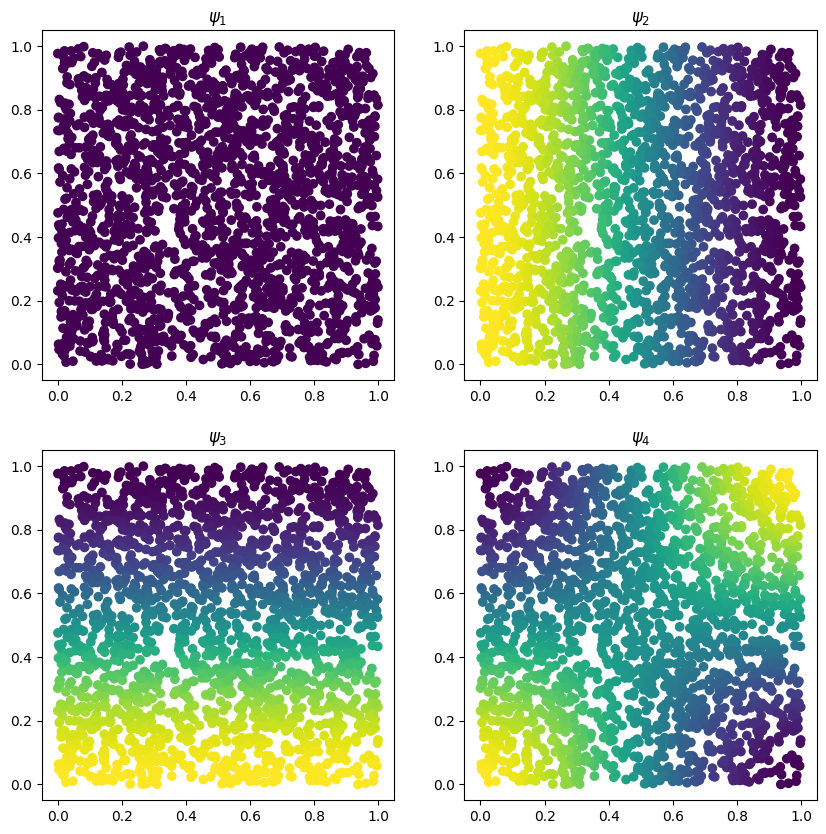
\includegraphics[width=14cm]{Fig2.jpg}
    \caption{Multiple scale expansion for different $\epsilon$ and $A$ values.}
\end{figure}

    \item Calculate the error 

    $$E(t) = |y_{numerical}(t)-y_{approximation}(t)|$$

    as a function of time ($0 \le t \le 40$) using $\epsilon = 0.01, 0.1, 0.2$ and $0.3$.

    \textbf{Solution:}
    \begin{figure}[H]
    \centering
    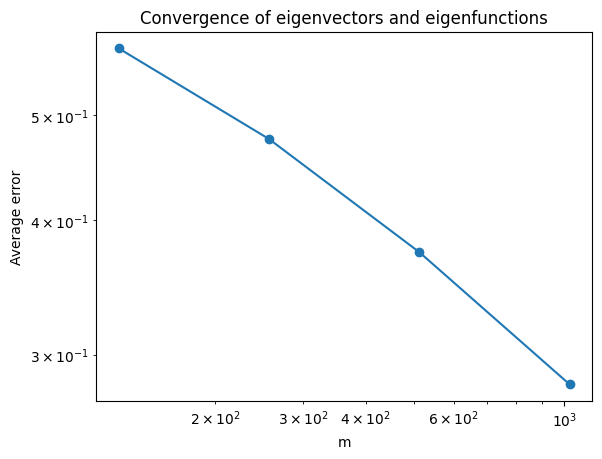
\includegraphics[width=14cm]{Fig3.jpg}
    \caption{Plot of the error between the numerical solution and the multiple scale approximation.}
\end{figure}
 \end{enumerate}

\end{enumerate}

\end{document}